%% This template can be used to write a paper for
%% Computer Physics Communications using LaTeX.
%% For authors who want to write a computer program description,
%% an example Program Summary is included that only has to be
%% completed and which will give the correct layout in the
%% preprint and the journal.
%% The `elsarticle' style is used and more information on this style
%% can be found at 
%% http://www.elsevier.com/wps/find/authorsview.authors/elsarticle.
%%
%%
\documentclass[preprint,12pt]{elsarticle}

%% Use the option review to obtain double line spacing
%% \documentclass[preprint,review,12pt]{elsarticle}

%% Use the options 1p,twocolumn; 3p; 3p,twocolumn; 5p; or 5p,twocolumn
%% for a journal layout:
%% \documentclass[final,1p,times]{elsarticle}
%% \documentclass[final,1p,times,twocolumn]{elsarticle}
%% \documentclass[final,3p,times]{elsarticle}
%% \documentclass[final,3p,times,twocolumn]{elsarticle}
%% \documentclass[final,5p,times]{elsarticle}
%% \documentclass[final,5p,times,twocolumn]{elsarticle}

%% if you use PostScript figures in your article
%% use the graphics package for simple commands
%% \usepackage{graphics}
%% or use the graphicx package for more complicated commands

\usepackage{graphicx}
\usepackage{subfigure}

%% or use the epsfig package if you prefer to use the old commands
%% \usepackage{epsfig}

%% The amssymb package provides various useful mathematical symbols
%% \usepackage{amssymb}
%% The amsthm package provides extended theorem environments
%% \usepackage{amsthm}

%% The lineno packages adds line numbers. Start line numbering with
%% \begin{linenumbers}, end it with \end{linenumbers}. Or switch it on
%% for the whole article with \linenumbers after \end{frontmatter}.
%% \usepackage{lineno}

%% natbib.sty is loaded by default. However, natbib options can be
%% provided with \biboptions{...} command. Following options are
%% valid:

%%   round  -  round parentheses are used (default)
%%   square -  square brackets are used   [option]
%%   curly  -  curly braces are used      {option}
%%   angle  -  angle brackets are used    <option>
%%   semicolon  -  multiple citations separated by semi-colon
%%   colon  - same as semicolon, an earlier confusion
%%   comma  -  separated by comma
%%   numbers-  selects numerical citations
%%   super  -  numerical citations as superscripts
%%   sort   -  sorts multiple citations according to order in ref. list
%%   sort&compress   -  like sort, but also compresses numerical citations
%%   compress - compresses without sorting
%%
%% \biboptions{comma,round}

% \biboptions{}

%% This list environment is used for the references in the
%% Program Summary
%%
\newcounter{bla}
\newenvironment{refnummer}{%
\list{[\arabic{bla}]}%
{\usecounter{bla}%
 \setlength{\itemindent}{0pt}%
 \setlength{\topsep}{0pt}%
 \setlength{\itemsep}{0pt}%
 \setlength{\labelsep}{2pt}%
 \setlength{\listparindent}{0pt}%
 \settowidth{\labelwidth}{[9]}%
 \setlength{\leftmargin}{\labelwidth}%
 \addtolength{\leftmargin}{\labelsep}%
 \setlength{\rightmargin}{0pt}}}
 {\endlist}

\journal{Computer Physics Communications}


\newcommand{\mytitle}{PLUMED-GUI: a visual environment to develop
  molecular dynamics analysis and biasing scripts}

\begin{document}

\begin{frontmatter}

%% Title, authors and addresses

%% use the tnoteref command within \title for footnotes;
%% use the tnotetext command for the associated footnote;
%% use the fnref command within \author or \address for footnotes;
%% use the fntext command for the associated footnote;
%% use the corref command within \author for corresponding author footnotes;
%% use the cortext command for the associated footnote;
%% use the ead command for the email address,
%% and the form \ead[url] for the home page:
%%
\title{\mytitle}
%% \tnotetext[label1]{}
\author{Toni Giorgino\corref{cor1}\fnref{label2}}
\ead{toni.giorgino@isib.cnr.it}
%% \ead[url]{home page}
%\fntext[label2]{Footnote}
\cortext[cor1]{To whom correspondence should be addressed}
\address{Institute of Biomedical Engineering (ISIB),\\ 
National Research Council of Italy (CNR),\\
Padua, Italy}
%\fntext[label3]{Label3}

%%\title{A \LaTeX{} template for CPC Computer Physics Descriptions}
%% use optional labels to link authors explicitly to addresses:
%% \author[label1,label2]{<author name>}
%% \address[label1]{<address>}
%% \address[label2]{<address>}

%% \author[a]{First Author\corref{author}}
%% \author[a,b]{Second Author}
%% \author[b]{Third Author}

%% \cortext[author] {Corresponding author.\\\textit{E-mail address:} firstAuthor@somewhere.edu}
%% \address[a]{First Address}
%% \address[b]{Second Address}

\begin{abstract}
  This paper presents PLUMED-GUI, an interactive environment to
  develop complex scripts for the Plumed molecular dynamics
  code. Plumed core provides a scripting language which can express a
  variety of collective variables and force-biasing
  protocols. PLUMED-GUI simplifies the development of analysis and
  biasing scripts for Plumed providing an integrated environment
  within the Visual Molecular Dynamics (VMD) software. In this way,
  computational biophysicists can leverage a richer syntax and
  interactive operations, for example leveraging VMD's
  chemically-based atom selection language.  Support for inserting the
  definition of common reaction coordinates is provided through
  pre-defined templates and syntax mnemonics; dialogs can be used to
  insert CV definitions which are often complex to create manually,
  such as extracting snapshots for RMSD or native contacts-based
  calculations.  PLUMED-GUI streamlines the development and test of
  analysis scripts, which can be computed on loaded trajectories
  within a VMD-based workflow, and therefore supports the rapid
  iteration of analysis and biasing scripts through incremental
  try-see-modify iterations.
\end{abstract}

% whose features include the ability to load and visualize
%  and manipulate multiple molecules and long trajectories.  

% its
%   scripting language, one can compute a wide range of collective
%   variables on existing molecular dynamics trajectories, or bias
%   simulations according to protocols such as metadynamics and
%   steering

%  make it an ideal environment to visualize and select parts of   complex molecular systems;

\begin{keyword}
Graphical User Interface \sep VMD \sep PLUMED \sep Molecular Dynamics \sep Collective Variables \sep Metadynamics 
\end{keyword}

\end{frontmatter}

%%
%% Start line numbering here if you want
%%
% \linenumbers

% Computer program descriptions should contain the following
% PROGRAM SUMMARY.

{\bf Program summary}
  %Delete as appropriate.

\begin{small}
\noindent
{\em Manuscript Title:}                                       
 \mytitle \\
{\em Authors:}                                                
 Toni Giorgino \\
{\em Program Title:}                                          
 VMD-PLUMED (Collective variable analysis plugin) \\
{\em Journal Reference:}                                      \\
  %Leave blank, supplied by Elsevier.
{\em Catalogue identifier:}                                   \\
  %Leave blank, supplied by Elsevier.
{\em Licensing provisions:}                                   
 3-clause BSD Open Source. \\
{\em Programming language:}                                   
 TCL/TK. \\
{\em Computer:}                                               
 Any capable of running  PLUMED [1] and VMD [2]. \\
{\em Operating system:}                                       
 Linux/Unix, OSX, Windows. \\
{\em RAM:}                                               
 As required to run  PLUMED [1] and VMD [2]. \\
{\em Number of processors used:}                              
 1 \\
% {\em Supplementary material:}                                 \\
  % Fill in if necessary, otherwise leave out.
{\em Keywords:} Graphical User Interface \sep VMD \sep PLUMED \sep Molecular Dynamics \sep Collective Variables \sep Metadynamics \\
  % Please give some freely chosen keywords that we can use in a
  % cumulative keyword index.
{\em Classification:}                                         
  3 Biology and Molecular Biology, 23 Statistical Physics and Thermodynamics. \\
% {\em External routines/libraries:}                            \\
  % Fill in if necessary, otherwise leave out.
{\em Subprograms used:}                                       
  PLUMED (version 1.3 or higher). \\
% {\em Catalogue identifier of previous version:}*              \\
  %Only required for a New Version summary, otherwise leave out.
% {\em Journal reference of previous version:}*                  \\
  %Only required for a New Version summary, otherwise leave out.
% {\em Does the new version supersede the previous version?:}*   \\
  %Only required for a New Version summary, otherwise leave out.
  {\em Nature of problem:} Compute and visualize values of collective
  variables on molecular-dynamics trajectories from within VMD and
  interactively develop biasing scripts for the estimation of
  free-energy surfaces in Plumed.
  \\
  {\em Solution method:} A graphical user interace is integrated in
  VMD and allows to interactively develop and run analysis scripts.
  Menus and dialogs provide mnemonics and documentation on the syntax
  to define complex CVs.
  \\
%{\em Reasons for the new version:}*\\
  %Only required for a New Version summary, otherwise leave out.
%{\em Summary of revisions:}*\\
  %Only required for a New Version summary, otherwise leave out.
  {\em Restrictions:}
  Tested on systems up to 100,000 atoms. \\
  {\em Unusual features:} VMD-PLUMED is not a standalone program but a
  VMD plugin that provides
  access to PLUMED's analysis features. \\
  {\em Additional comments:} Distributed with VMD since version 1.9.0.
  Update manually to access   the latest features.   \\
  {\em Running time:} Depends on the size of the system and the length
  of the trajectory; usually negligible with respect to simulation time.  \\
\begin{thebibliography}{0}
\bibitem{1}See paper in this issue.
\bibitem{2}Humphrey, W., A. Dalke, and K. Schulten. ``VMD: Visual Molecular Dynamics.'' J Mol Graph 14, no. 1 (February 1996): 33-38. 
\end{thebibliography}

%* Items marked with an asterisk are only required for new versions
%of programs previously published in the CPC Program Library.\\
\end{small}



\section{Introduction}



- large scale simulations becoming commonplace

- reactions can be described as long as one has good reaction coordinates

- RC can be used post-hoc for analysis

- need methods to test collective variable definitions

- when one has a trajectory, he wants to be quickly get the value of given CVs over it

- CV can be quite sophisticated / see plumed 

-- however, they have to be defined with chemical awareness

-- this implies taking into account topologies

-- for example expressing lists of atoms as quasi-natural-language expressions

-- DRIVER


\section{Plugin usage}

The main PLUMED-GUI interface is opened selecting the
``Analysis/Collective variable analysis (PLUMED)'' entry found under
VMD Main window's Extensions menu. Overall, the interface
(Figure~\ref{fig:main}) behaves like a text editor; in fact, File and
Edit menus provide the customary editing commands, verbatim file read
and write functions, and undo/redo.  Upon start, the text area holds a
short syntax reminder, which can be dismissed if desired. The Plumed
script is edited in the main text area.  The script should follow the
syntax of the Plumed version currently in use.

The analysis is started by pressing the ``Plot'' button at the bottom
of the window. Assuming that Plumed executable is properly installed,
the GUI will invoke Plumed's ``driver'' function, which will evaluate
the collective variables defined in script on each of the trajectory
frames of the currently selected system (known in VMD as the
\emph{top} molecule).

Once the evaluation is complete, a plot is displayed with the time
series of the collective variables, each shown with a different color.
The purpose of the plot is to quickly inspect the values yielded by
the current CV definition, and provide a quick way to iterate and
refine them.  If a more advanced layout is desired, the numeric data
can be exported from the plot window either as a matrix (with rows
being time, and columns as CVs), or as 1-D timeseries separated by
empty lines.

It is important to note that the GUI does not restrict the syntax
available to the user; the script is passed as-is to the underlying
driver, with the sole exception of expanding symbolic expressions in
square brackets, which will be discussed in the next section.

Should the script generate errors, these displayed in VMD console.  If
driver identifies the line containing the error, the error is
highlighted with a red background in the text input area.






\begin{figure}
  \centering
  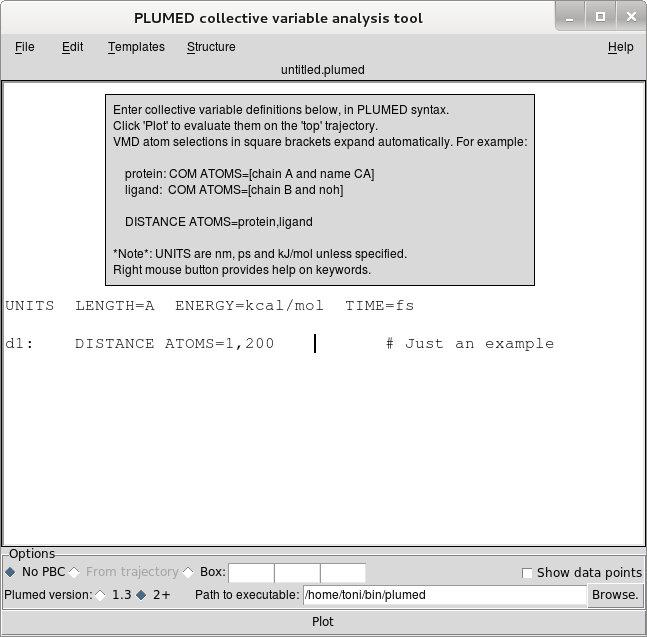
\includegraphics[width=0.8\textwidth]{images/main}
  \caption{PLUMED-GUI's main window. 
    The analysis script is entered in the text area, which behaves as
    a text editor; shortcuts accessible from the ``Templates'' menu
    insert frequently-used definitions. The ``Plot'' button evaluates
    the script on the currently-selected (``top'') trajectory, and, if
    successful, displays a graph showing the values of the chosen
    collective variables at each frame. The gray box, only shown at
    startup, contains a brief reminder on the use of the interface.  }
  \label{fig:main}
\end{figure}


\subsection{Using symbolic atom selections}


\subsection{Templates}


\subsection{On-line help}

Plumed's action syntax provides a wealth of options for specifying the
behavior of CVs. For example, the simple \texttt{DISTANCE} action
foresees modifiers to compute derivatives numerically, to ignore
periodic boundary conditions, and/or to return the components of the
distance vector rather than its modulus. The richness of the syntax
may make it difficult to remember all of the supported keywords and
default values.  Although templates include placeholders for most
common options, it would be impractical to include all of the optional
parameters in each template line.

PLUMED-GUI provides context-sensitive syntax reminders through a
pop-up menu, invoked pressing the right mouse button on an action
keyword (Figure~\ref{fig:help}).


\begin{figure}
  \centering
  \subfigure{
    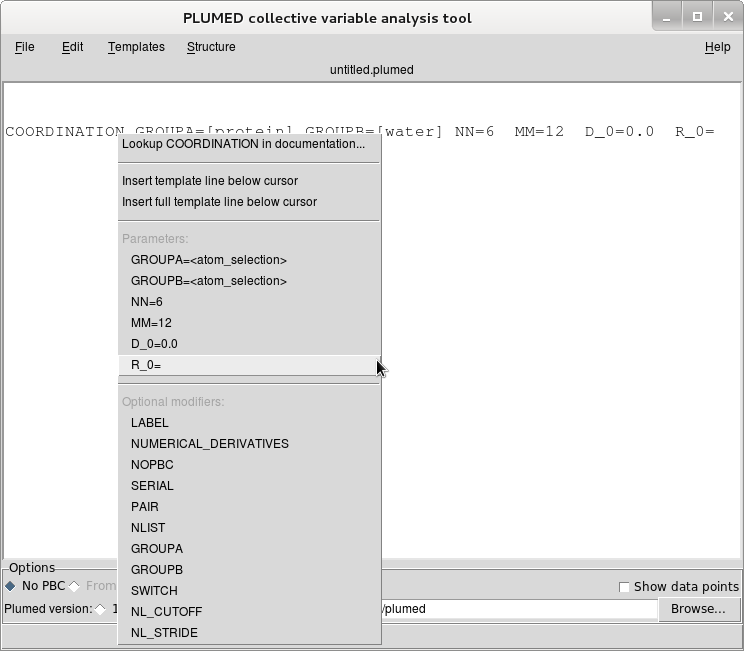
\includegraphics[width=0.5\textwidth]{images/help_popup}
  }
  \subfigure{
    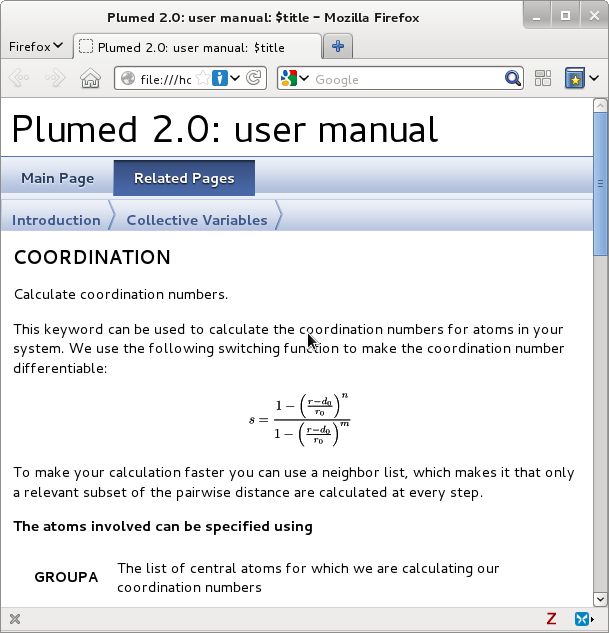
\includegraphics[width=0.4\textwidth]{images/help_page}
  }    
  \caption{(a) A contextual popup menu lists the mandatory and
    optional keywords supported by the action under the pointer (in
    this case, \texttt{COORDINATION}, which computes the coordination
    number of one or two groups of atoms). (b) The ``Lookup'' function
    displays the action's manual in a web browser. }
  \label{fig:help}
\end{figure}

\subsection{Analysis and visualization}

Export data as matrix and ...

Point readout




\section{Structure-based commands}

%The \textit{Structure} menu supports the construction of complex CVs.

Some CVs require too much information to be defined by one script command.
The objective of the \emph{Structure} menu is to provide assistance in the declaration of CVs
that depend upon the topology and coordinates of the currently loaded
system. Such CVs generally involve long lists of statements and/or
auxiliary files; automated procedures therefore relieve users
from the cumbersome and error-prone process of building these lists by
hand. Each of the functions provided in the menu opens a dialog where
it is possible to tune the options for the CV being defined.

\begin{figure}\label{fig:structure}
  \centering
  \subfigure[Build reference structure]{
    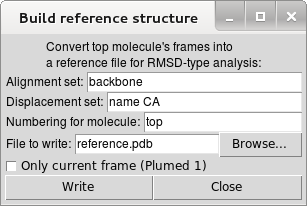
\includegraphics[scale=.4]{images/reference} \label{fig:reference}}
  \subfigure[Native contacts]{
    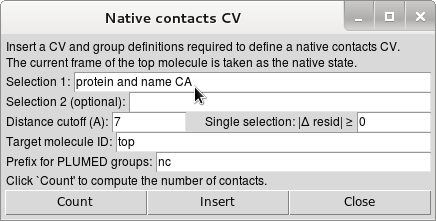
\includegraphics[scale=.4]{images/native} \label{fig:native}}
  \subfigure[Ramachandran angles]{
    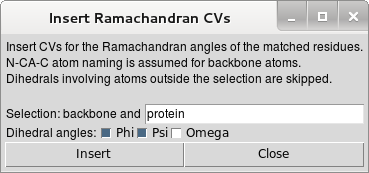
\includegraphics[scale=.4]{images/rama} \label{fig:rama}}
  \caption{Entries in the ``Structure'' menu support the creation of
    CVs based on the active topology; each opens up a dialog, as shown
    above. (a) ``Build reference structure'' creates a reference file
    for RMSD-based calculations on the basis of the currently
    displayed frame. Displacement and alignment sets can be specified
    as VMD atom selections; numbering can be mapped between molecules
    if the reference frame and the trajectory on which to compute the
    CV have different topologies. (b) ``Native contacts'' computes the
    list of atom pairs (which are within the chosen distance) in the
    currently-displayed (``native'') frame. The CV will consist in
    counting how many of these contacts are present at each time
    instant.  Contacts between neighboring residues can be filtered
    out providing a lower bound to the $| \Delta \mbox{resid} |$
    parameter. (c) The ``Ramachandran angles'' dialog inserts CVs that
    compute $\phi, \psi$ and/or $\omega$ dihedral angles contained in
    the selection.}
\end{figure}

\subsection{Reference structures for alignments}

A typical example of a CV which requires structural data for its
definition, and thus more information than contained in the script, is
the root mean square deviation (RMSD) of a set of atoms with respect
to a reference frame. RMSD are computed averaging the squared
displacement of a chosen set of atoms (displacement set) after finding
the roto-translation that optimally aligns another, possibly
coincident, set of atoms (alignment set). 

Plumed allows the selection of the two sets and the reference
coordinates through ``reference files'', which encode - in PDB-like
syntax - the subset of atoms to be considered, and whether each
belongs to the displacement and/or alignment set. 

The ability to readily generate reference files is especially
important because they are employed in a useful generalization of the
RMSD metric, namely the $S$ and $Z$ path
variables~\cite{Branduardi_Gervasio_Parrinello_2007}.  Path variables
which express the ``progression'' and ``distance'' of the current
state of the system along a path defined by a number of exemplary
structures used as landmarks.



\subsection{Native contacts}




\subsection{Ramachandran angles}




\subsection{Export for use in simulation}

In addition to computing CVs on pre-computed trajectories, Plumed is
often used to bias simulations through forces that enhance the
sampling of the phase-space in a way that allows the reconstruction of
free-energy surfaces. 

Simulations are executed in MD codes, patched in order to take into
account the force biases specified by the user in the plumed script;
such scripts include the CVs to be biased, and the biasing protocol
(e.g. constraining elastically CVs to a given value, steering them to
increasing or decreasing values, metadynamics, and so on).  Plumed
core only allows the atoms to be specified through their serial
number; therefore, developing biasing scripts can become an
error-prone exercise in presence of numerous CVs and complex atom
specifications.  

The ``export'' function, found in the File menu,  substitutes all the
symbolic atom selections in the current script with the corresponding
numerical lists; the script thus exported can be then used in
simulation.  For the sake of reproducibility and reference, it is
generally useful to preserve both the exported file and the original
script (with unsubstituted, symbolic atom selections). However, if the
latter is lost, the exported file still contains comments which remind
how the atom lists were computed.




\section{Installation}

Recent VMD distributions contain a preinstalled version of PLUMED-GUI.
This paper describes version 2.0 of the GUI, which supports Plumed 2.0
and earlier.  Users may manually update their GUI to the latest
version.



\subsection{Compatibility} 

The GUI supports the same wide range of platforms as VMD, encompassing
all major variants of Linux/Unix, OSX, and Windows. To analyze
trajectories, the plugin executes Plumed's ``driver'' binary for the
platform; on Unix-like systems, such binary is obtained following the
instructions included in Plumed's distribution; a precompiled version
for Windows is provided for convenience.

The language syntax and invocation method differ between Plumed
versions 2.0 and 1.3.  The GUI detects which version is installed upon
start, and adapts templates and syntax accordingly.  If both plumed
versions are available, the user can switch manually between the two.


\subsection{Consistency of units}

It may be worth noting that the units of computed CVs only depends on
Plumed's conventions.  Since version 2.0, Plumed defaults to the
nanometer, kJ/mol, picosecond combination. Given that VMD users
may be accustomed to the \AA ngstrom, kcal/mol, femtosecond unit
set, a reminder is shown about the fact that they can use Plumed's
\texttt{UNITS} keyword to switch to customary units.


\subsection{Version and updates}

The current version of the plugin, PLUMED-GUI 2.0, supports both
Plumed 1.3 and Plumed 2.0, with minor functional differences. For
clarity, this paper only discusses the features available when the GUI
is used along with Plumed 2.0.

To update the GUI, it is sufficient to identify VMD's installation
path, and replace the files contained in the subdirectory named
\verb+plugins/noarch/tcl/plumed+ with those in the latest
distribution.  As customary, the ``About'' menu item displays the
currently installed version of the GUI.




\section{Conclusions}

This paper described the functions of a graphical interface to develop
scripts for the Plumed molecular dynamics software. The interface
integrates into a well-known ``host'' molecular visualization program,
VMD\cite{Humphrey_Dalke_Schulten_1996}, leveraging its facilities in terms of ease of loading multiple
systems and long trajectories at the same time, plotting, and a
powerful chemically-aware atom selection language. At the same time,
the underlying Plumed code provides both the mathematical facilities
and a uniform, straightforward syntax to express a wide range of
collective variables used in the practice of molecular simulations.
In this sense, PLUMED-GUI merges the best of both worlds -- the
usability of a graphical interface and the expressiveness of Plumed's
powerful CV description language.

Limitations?



\section{Acknowledgements}

Part of the work described in this paper was conducted while at the
Computational Biophysics Laboratory at the Universitat Pompeu Fabra
(Barcelona). Support from the ''Beatriu de Pinos'' scheme of the
Generalitat de Catalunya is gratefully acknowledged.




%% References with bibTeX database:

\bibliographystyle{elsarticle-num}
\bibliography{colvar}



\end{document}

;; %%% Local Variables:
;; %%% TeX-command-default: "Make"
;; %%% mode: latex
;; %%% TeX-master: "masterfile"
;; %%% End: 


